\chapter{Stato dell'arte}
\label{cha:statoArte}

\section{Reverse Proxy}
\subsection{Cos'é}
Un reverse proxy é un dispositivo che fa da intermediario tra i server presenti sotto una rete locale e la rete esterna. Le comunicazioni in uscita dai server passano quindi dal reverse proxy e poi vanno verso gli utenti, e uguale quelle in ingresso, entrano nella rete locale attraverso il reverse proxy e poi vengono indirizzate ai server desiderati.
\begin{figure}[h!]
  \centering
  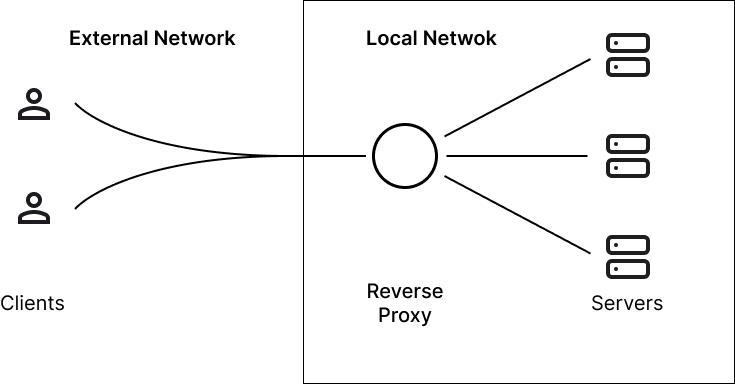
\includegraphics[width=.6\textwidth]{images/schema.png}
\end{figure}

\subsection{Perché viene utilizzato}
L'utilizzo di una struttura che si pone in mezzo alle comunicazioni garantisce molti vantaggi visto che ha accesso a tutte le comunicazioni entranti. Il reverse proxy puó quindi analizzare le connessioni ed effettuare delle operazioni con queste ultime come ad esempio controlli per motivi di sicurezza, chaching e  load balancing. Inoltre in questo modo si puó accedere a piú servizi tramite lo stesso nodo di ingresso.

\subsection{Funzionalitá}
Analizziamo adesso le funzionalitá che un reverse proxy puó offrire.

\subsubsection{Sicurezza}
Sicuramente le funzionalitá piú importanti sono quelle relative alla sicurezza. Un reverse proxy infatti ne implementa molte evitando la necessitá di implementare sistemi di sicurezza per ogni servizio che andiamo ad inserire nella rete locale.
\begin{enumerate}
  \item \textbf{TLS}: Ogni comunicazioni in ingresso e in uscita puó essere criptata tramite il protocollo TLS.

\end{enumerate}


